% Векторизация римановского решателя.
\subsection{Векторизация гнезд циклов с непостоянным количеством итераций}

\cite{Rybakov2019VecRiem1} \cite{Rybakov2019VecRiem2}

\subsubsection{Описание римановского решателя}

Рассматриваемая в данной статье реализация римановского решателя находится в открытом доступе в сети Интернет в составе библиотеки NUMERICA \cite{Numerica}.
Нас в данном случае будет интересовать одномерный случай для однокомпонентной среды, реализованный в виде чистой функции (функции без побочных эффектов, результат работы функции зависит только от значений входных параметров), которая по значениям плотности, скорости и давления газа слева и справа от разрыва, находит значения этих же величин на самом разрыве в нулевой момент времени после устранения перегородки.

\begin{equation}\label{eq:riemann}
U_l = \left( \begin{array}{ccc} d_l \\ u_l \\ p_l \end{array} \right),
U_r = \left( \begin{array}{ccc} d_r \\ u_r \\ p_r \end{array} \right),
U = \left( \begin{array}{ccc} d \\ u \\ p \end{array} \right) = riem(U_l, U_r)
\end{equation}

В формуле (\ref{eq:riemann}) через $d_l$, $u_l$, $p_l$ обозначены плотность, скорость и давление газа слева от разрыва (они объединены в структуру  $U_l$ -- состояние газа слева от разрыва).
Аналогично через $d_r$, $u_r$, $p_r$ обозначены плотность, скорость и давление газа справа от разрыва, объединенные в состояние газа $U_r$.
Переменными $d$, $u$, $p$ обозначены плотность, скорость и давление газа, полученные в результате решения задачи Римана.

Библиотека NUMERICA реализована на языке программирования FORTRAN, поэтому векторизация данного кода с использованием функций-интринсиков напрямую невозможна, поэтому использовалась портированная на язык программирования C версия кода.

\begin{figure}
\centering
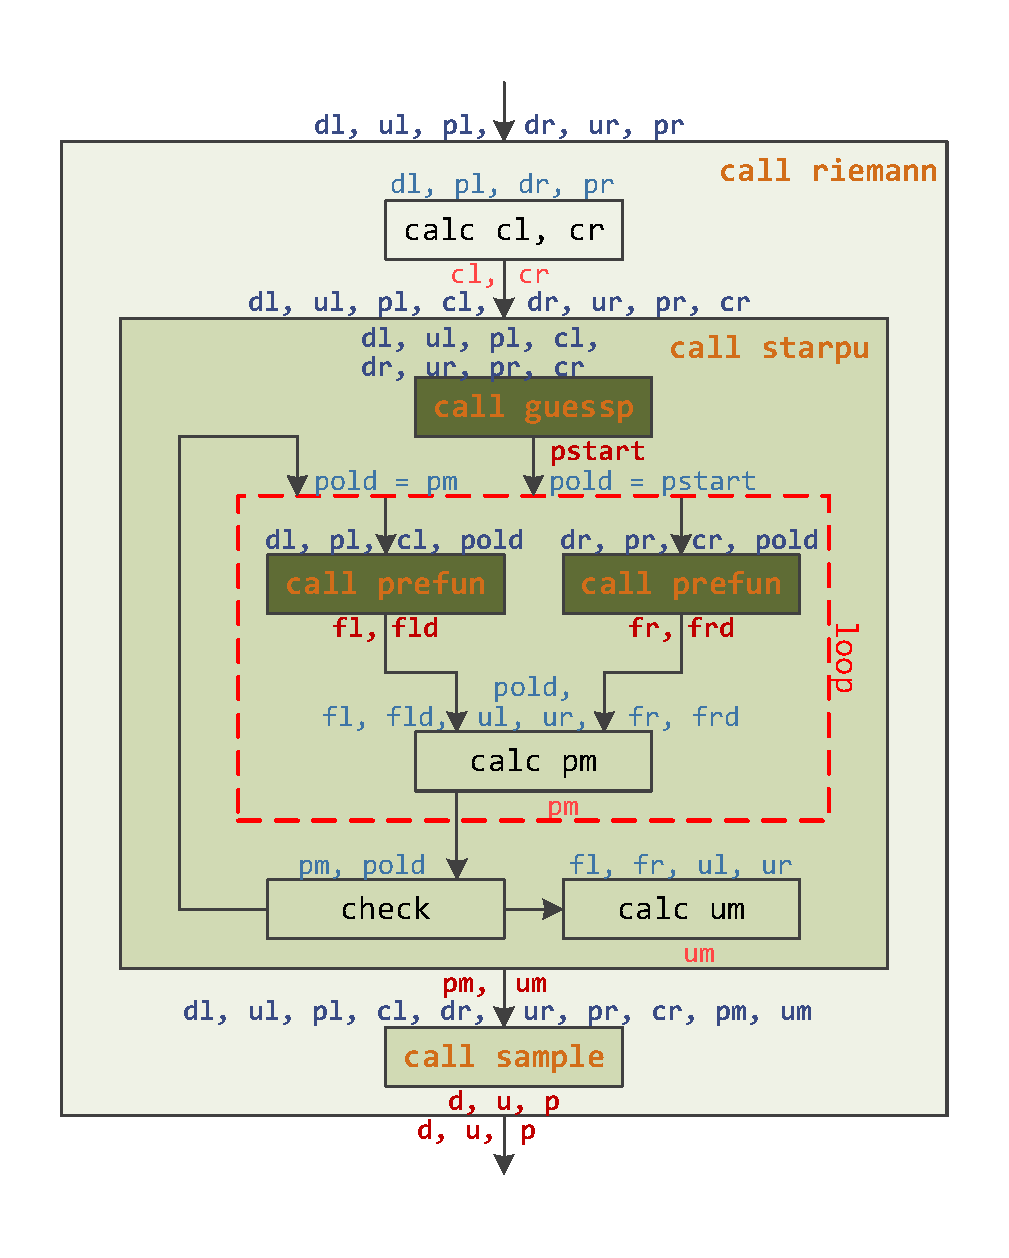
\includegraphics[width=0.8\textwidth]{pics/text_4_vec_riemann/pic_functions.pdf}
\caption{Схема потока данных в римановском решателе}
\label{pic:functions}
\end{figure}

На Рис.~\ref{pic:functions} показана схема работы римановского решателя с обозначенными потоками данных и вызовами всех входящих в реализацию функций. Функция \texttt{riemann} осуществляет вычисление скорости звука справа и слева, выполняет проверку на образование вакуума и последовательно вызывает функции \texttt{starpu} и \texttt{sample}.
Функция \texttt{starpu} вычисляет значения скорости и давления в среднем регионе между левой и правой волнами (star region), при этом функция содержит цикл с неизвестным количеством итераций для решения нелинейного уравнения итерационным методом Ньютона, внутри которого расположены вызовы других функций (\texttt{prefun}).
Функции \texttt{guessp} и \texttt{prefun} содержат только арифметические вычисления и простые условия и являются наиболее простыми с точки зрения векторизации.
Наконец последняя функция sample определяет окончательную конфигурацию разрыва путем вычисления множества условий.
Данная функция содержит очень разветвленное управление, вложенность условий в ней достигает четырех, что затрудняет применение векторизации.

В процессе счета с помощью численных методов, базирующихся на римановском решателе, выполняется множество вызовов функции \texttt{riemann} с различными наборами входных данных (на каждой итерации счета выполняется один вызов для каждой грани каждой ячейки расчетной сетки).
Так как функция riemann является чистой, то вызовы для разных наборов входных данных (\texttt{dl}, \texttt{ul}, \texttt{pl}, \texttt{dr}, \texttt{ur}, \texttt{pr}) являются независимыми и возникает желание объединения вызовов с целью эффективного задействования векторных (поэлементных) инструкций.
В качестве такого объединенного вызова будем рассматривать функцию, в которую вместо атомарных данных типа \texttt{float} будут подаваться соответствующие векторы, содержащие по 16 элементов.

\begin{equation}\label{eq:riemann_16}
\overline{U_l} = \left( \begin{array}{ccc} \overline{d_l} \\ \overline{u_l} \\ \overline{p_l} \end{array} \right),
\overline{U_r} = \left( \begin{array}{ccc} \overline{d_r} \\ \overline{u_r} \\ \overline{p_r} \end{array} \right),
\overline{U} = \left( \begin{array}{ccc} \overline{d} \\ \overline{u} \\ \overline{p} \end{array} \right) = riem(\overline{U_l}, \overline{U_r})
\end{equation}

В формуле (\ref{eq:riemann_16}) все переменные $\overline{d_l}$, $\overline{u_l}$, $\overline{p_l}$, $\overline{d_r}$, $\overline{u_r}$, $\overline{p_r}$, $\overline{d}$, $\overline{u}$, $\overline{p}$ являются векторами длины 16.
Например, вектор $\overline{d}$ содержит 16 значений плотности газа, полученных при решении 16 задач Римана, объединенных в один вызов.
Аналогично с другими переменными.

При этом с векторными данными можно производить те же действия, что и с базовыми типами -- выполнять вычисления, передавать в функции, возвращать в качестве результата.
В процессе оптимизации для наглядности будем избегать подстановки тела функции в точку вызова.
Таким образом, в результате векторизации нашей целью является получение векторных аналогов всех используемых в римановском решателе описанных выше функций.

Простой контекст -- prefun.
Сильно разветвленные условия -- sample.

\subsubsection{Векторизация гнезда циклов}

\begin{figure}
\centering
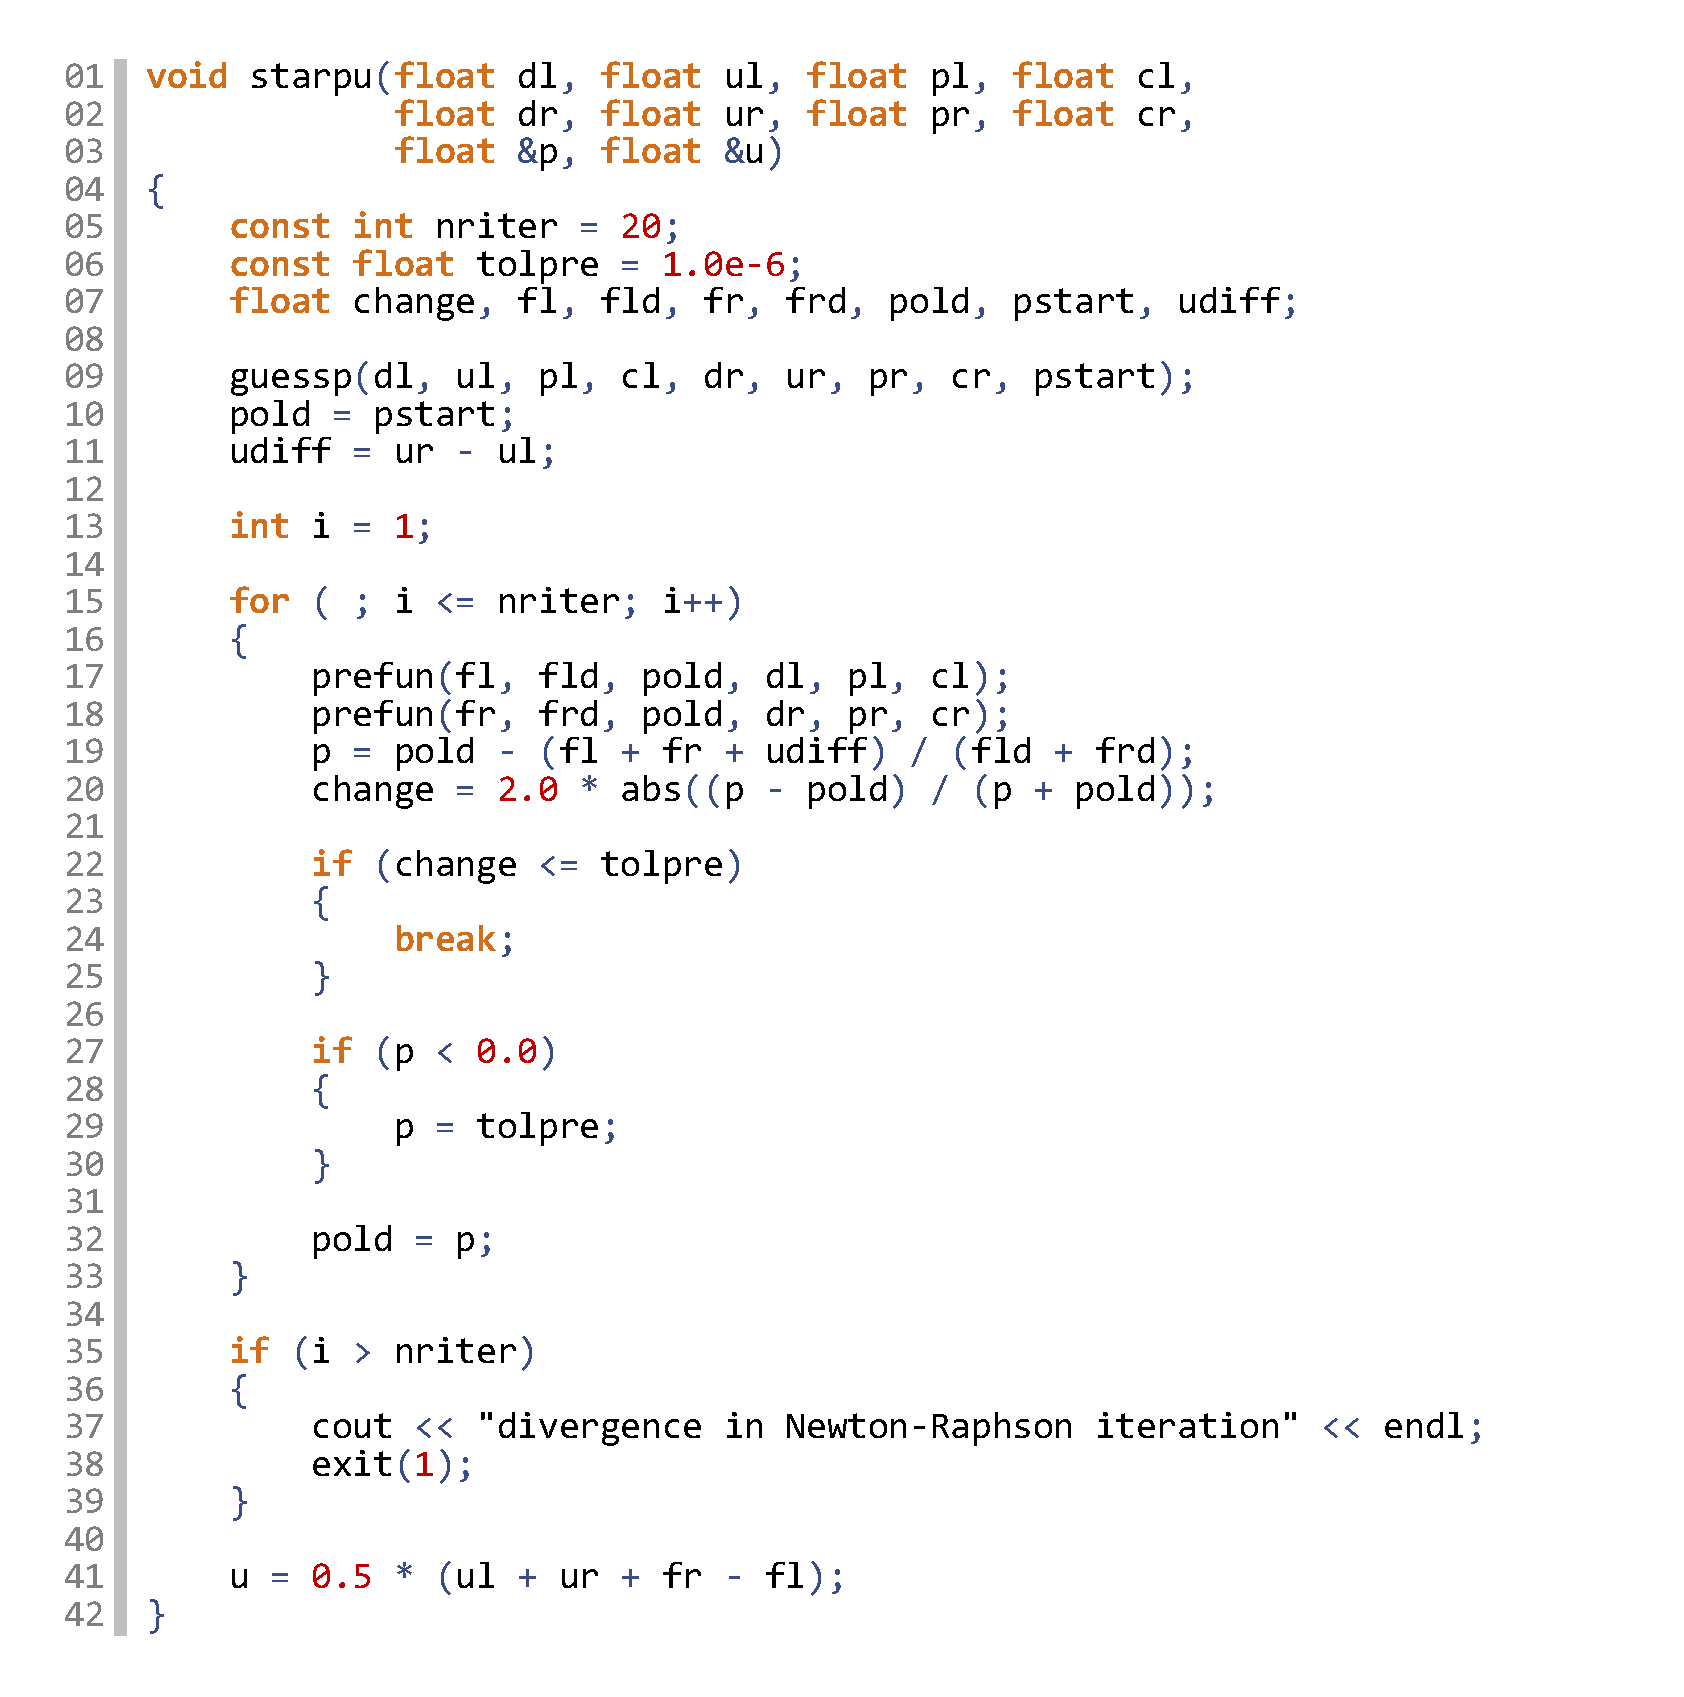
\includegraphics[width=0.8\textwidth]{pics/text_4_vec_riemann/pic_starpu_code.pdf}
\caption{Оригинальная версия функции \texttt{starpu}}
\label{pic:starpu_code}
\end{figure}

Наиболее сложным контекстом для векторизации кода является функция \texttt{starpu}, содержащая цикл с неизвестным количеством итераций (Рис.~\ref{pic:starpu_code}).
Цикл, расположенный в данной функции в строках 15-33 кроме неизвестного количества итераций содержит также условные переходы (\texttt{if, break}) и вызовы функций prefun, что также усложняет его векторизацию.
Перед выполнением векторизации данный цикл необходимо преобразовать в предикатную форму, в которой тело не должно содержать операций перехода.
Все инструкции цикла выполняются под своими предикатами, а выполнение цикла прерывается при условии обнуления всех предикатов.
Данный механизм описан в работе \cite{RybTelShabLoopsVect} применительно к векторизации сортировки Шелла, а также в \cite{Krzikalla} применительно к построению множества Мандельброта.
При этом стоит заметить, что вызовы функций prefun также должны обладать соответствующими предикатами.
После преобразования тела цикла в предикатную форму, он может быть векторизован, после чего предикаты инструкций заменятся на векторные регистры-маски (именно в этом месте появляется дополнительный параметр векторизованной функции \texttt{prefun} в виде маски).
Результат векторизации функции \texttt{starpu} представлен на Рис.~\ref{pic:starpu_16_code}.
В строке 18 видна изначальная инициализация полной маски выполнения векторизованных итераций цикла. По мере работы цикла маска истощается (строка 32), и при полном ее обнулении цикл завершает работу.

\begin{figure}
\centering
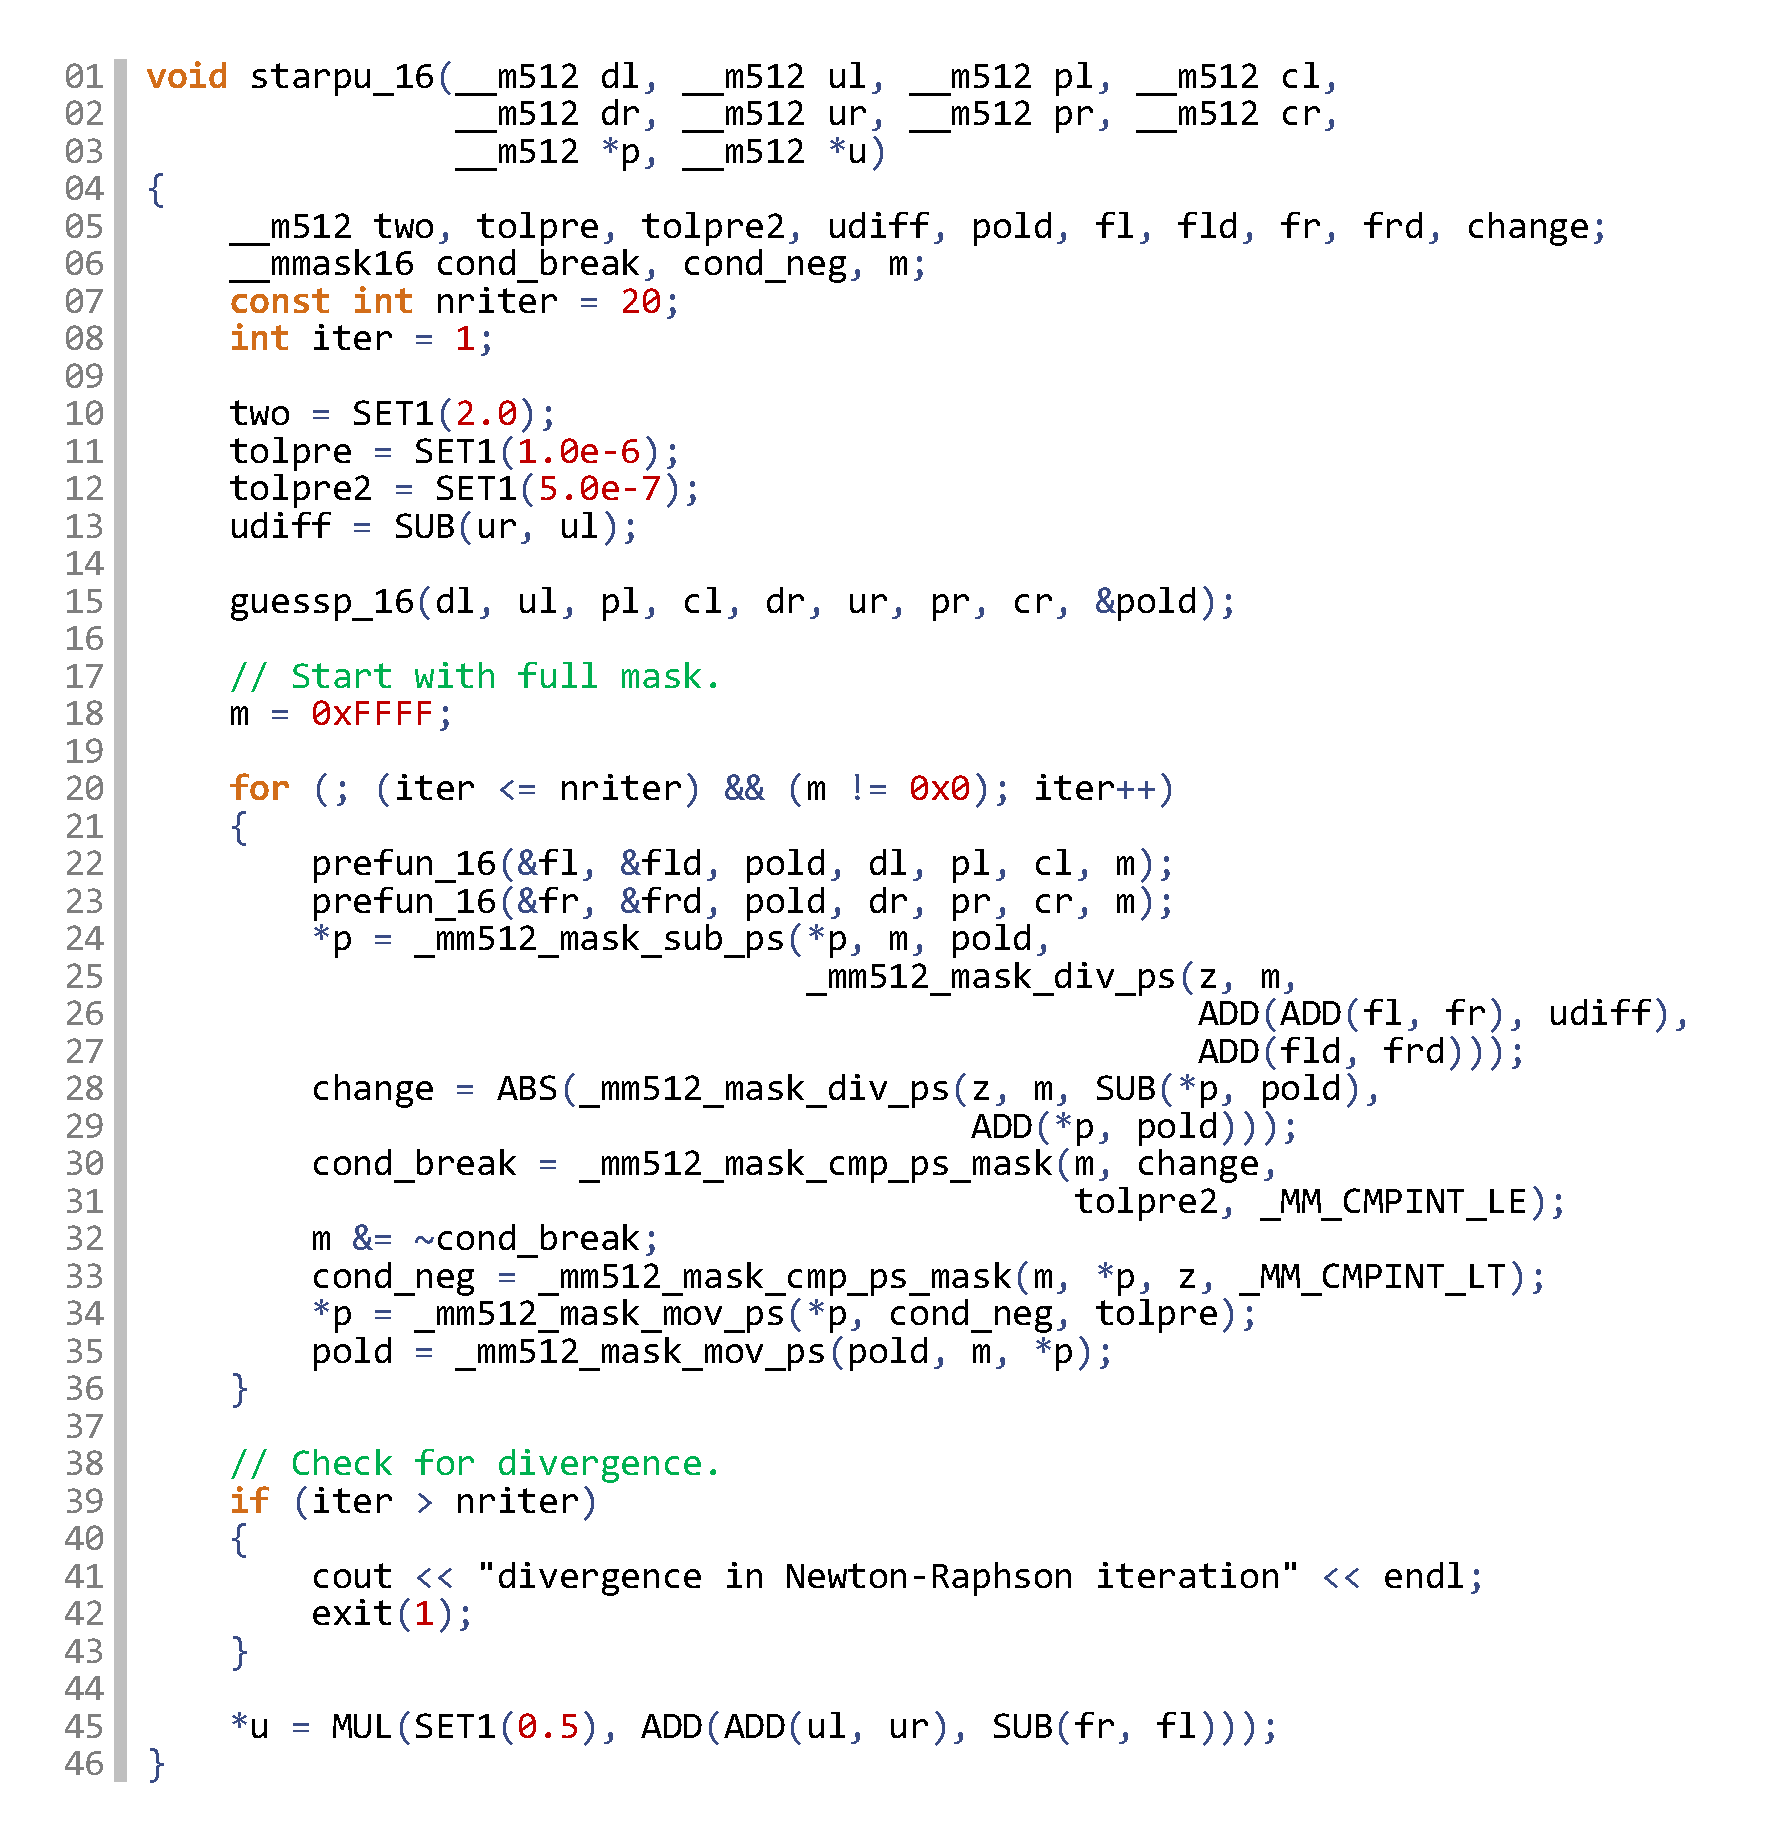
\includegraphics[width=0.8\textwidth]{pics/text_4_vec_riemann/pic_starpu_16_code.pdf}
\caption{Векторизованная версия функции \texttt{starpu}}
\label{pic:starpu_16_code}
\end{figure}

Стоит отметить, что векторизация цикла с неизвестным числом итераций может быть довольно опасной, так как количество итераций векторизованного цикла равно максимуму из количеств итераций циклов из 16 объединяемых вызовов оригинальной невекторизованной функции.
При большой разнице в количестве итераций оригинального кода возникает падение эффективности, связанное с низкой плотностью масок исполняемых инструкций, как это показано в работе \cite{RybTelShabLoopsVect}.

\subsubsection{Анализ результатов}

Перед началом оптимизации программного кода римановского решателя был выполнен сбор профиля исполнения, который показал, что время исполнения распределено между отдельными функциями согласно диаграмме, представленной на Рис.~\ref{pic:exe_prof}.

\begin{figure}
\centering
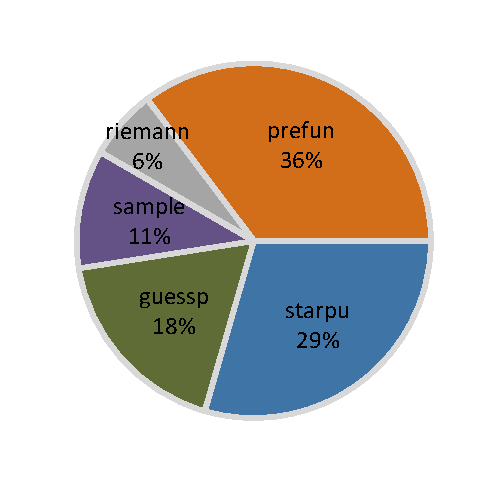
\includegraphics[width=0.4\textwidth]{pics/text_4_vec_riemann/pic_exe_prof.pdf}
\caption{Распределение времени выполнения римановского решателя между отдельными функциями}
\label{pic:exe_prof}
\end{figure}

Для сбора профиля исполнения исходная программа была скомпилирована с запретом оптимизации подстановки тела функции в точку вызова (inline).
Таким образом, на диаграмме отмечено чистое время выполнения функций без учета вложенных вызовов.
Из диаграммы видно, что наибольшая доля времени исполнения приходится на функцию \texttt{prefun} (36\%), содержащую простой программный контекст с одним условием.
Также значительная часть времени исполнения приходится на функцию \texttt{starpu} (29\%), содержащую гнездо циклов с неизвестным числом итераций.
Оставшееся время делится между тремя другими функциями \texttt{guessp} (18\%), \texttt{sample} (11\%), \texttt{riemann} (6\%).

Описанные в статье подходы к векторизации функций римановского решателя были реализованы на языке программирования C с использованием функций-инстринсиков и опробованы на микропроцессорах Intel Xeon Phi 7290, входящих в состав вычислительного сегмента knl суперкомпьютера МВС-10П, находящегося в МСЦ РАН.

Тестирование производительности выполнялось на массивах входных данных, собранных при решении стандартных тестовых задач: задача Сода, задача Лакса, задача о слабой ударной волне, задача Эйнфельдта, задача Вудворда-Колелла, задача Шу-Ошера и других \cite{BulVolTest}.

На диаграмме Рис.~\ref{pic:perf} показан эффект от применения различных оптимизаций к каждой из рассматриваемых функций, а также суммарное ускорение, полученное вследствие векторизации.

\begin{figure}
\centering
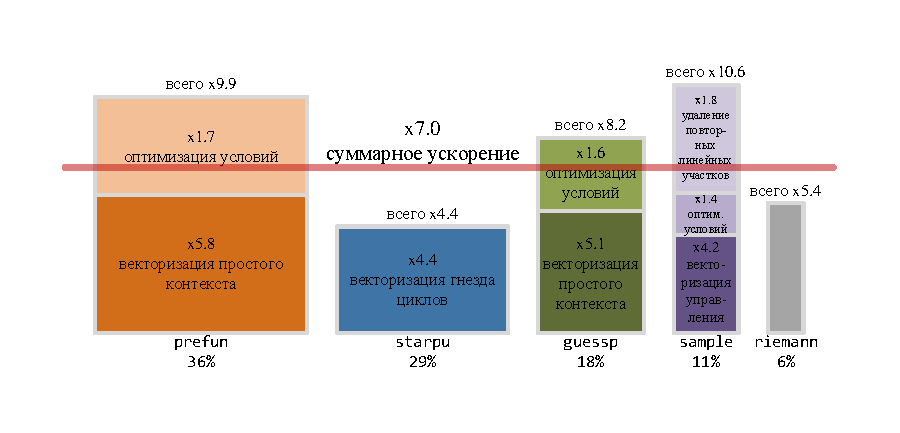
\includegraphics[width=1.0\textwidth]{pics/text_4_vec_riemann/pic_perf.pdf}
\caption{Диаграмма ускорения отдельных функций и суммарного ускорения римановского решателя}
\label{pic:perf}
\end{figure}

Можно отметить, что эффект от векторизации простого контекста варьируется в пределах от 5.1 до 5.8 раза (для функций \texttt{guessp} и \texttt{prefun}).
Также следует отметить существенный эффект от оптимизации условий (проверка на пустоту маски предикатов, под которой находится выполнение блока операций).
Это довольно простое преобразование, приводит к ускорению кода от 1.4 до 1.7 раз (для функций \texttt{sample} и \texttt{prefun}) в зависимости от того, насколько близкими являются условия с соседних итераций векторизуемого цикла.

Отдельно на диаграмме выделен эффект от применения оптимизации замены переменных, позволившей в 1.8 раз ускорить функцию \texttt{sample} путем слияния двух поддеревьев графа потока управления (то есть было выполнено удаление дублирующих линейных участков).

В результате применения всех описанных оптимизаций удалось достичь ускорения отдельных участков выполнения программы в 10 и более раз, а суммарное ускорение всего римановского решателя составило 7 раз (отмечено красной линией на Рис.~\ref{pic:perf}).